\documentclass[tikz,border=10pt]{standalone}
\usepackage{tikz}
\usetikzlibrary{shapes.geometric}

\begin{document}
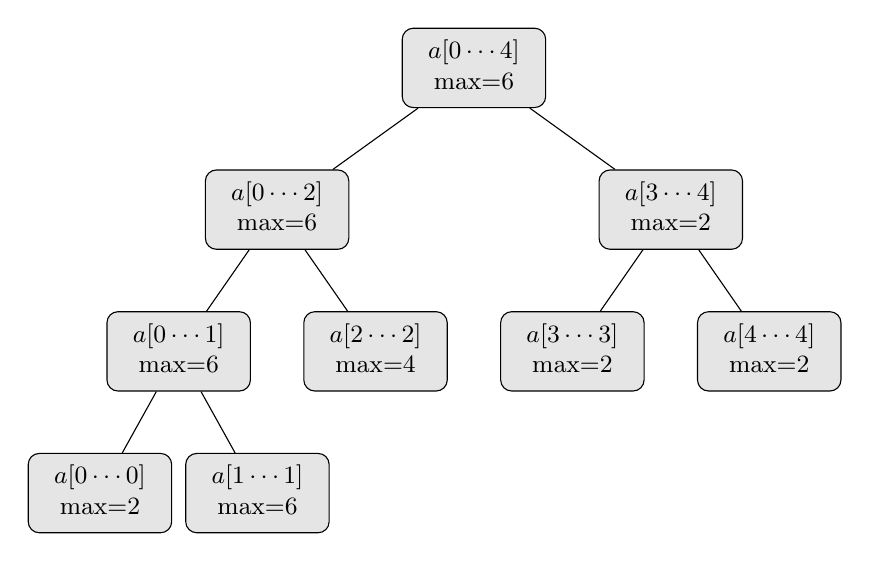
\begin{tikzpicture}[
  level distance=1.8cm, % Increased distance between levels
  edge from parent/.style={draw}, % Removed arrowheads
  every node/.style={rectangle, rounded corners, draw=black, fill=gray!20, text centered, text=black, font=\small},
  level 1/.style={sibling distance=5cm}, % Wider spacing for first level
  level 2/.style={sibling distance=2.5cm}, % Moderate spacing for second level
  level 3/.style={sibling distance=2cm} % Adjusted spacing for the third level
]

% Root node
\node {%
  \begin{tabular}{c}
    $a[0 \cdots 4]$ \\
    max=6
  \end{tabular}
}
  % Level 1
  child {node {%
    \begin{tabular}{c}
      $a[0 \cdots 2]$ \\
      max=6
    \end{tabular}
  }
    % Level 2 (left subtree)
    child {node {%
      \begin{tabular}{c}
        $a[0 \cdots 1]$ \\
        max=6
      \end{tabular}
    }
      % Level 3 (left subtree of left subtree)
      child {node {%
        \begin{tabular}{c}
          $a[0 \cdots 0]$ \\
          max=2
        \end{tabular}
      }}
      child {node {%
        \begin{tabular}{c}
          $a[1 \cdots 1]$ \\
          max=6
        \end{tabular}
      }}
    }
    child {node {%
      \begin{tabular}{c}
        $a[2 \cdots 2]$ \\
        max=4
      \end{tabular}
    }}
  }
  child {node {%
    \begin{tabular}{c}
      $a[3 \cdots 4]$ \\
      max=2
    \end{tabular}
  }
    % Level 2 (right subtree)
    child {node {%
      \begin{tabular}{c}
        $a[3 \cdots 3]$ \\
        max=2
      \end{tabular}
    }}
    child {node {%
      \begin{tabular}{c}
        $a[4 \cdots 4]$ \\
        max=2
      \end{tabular}
    }}
  };

\end{tikzpicture}
\end{document}